%!TEX root = ../Thesis.tex
% Chapter Template

\chapter{Theory} % Main chapter title
\label{Theory} % Change X to a consecutive number; for referencing this chapter elsewhere, use \ref{ChapterX}
\lhead{Chapter \ref{Theory}. \emph{Theory}} % Change X to a consecutive number; this is for the header on each page - perhaps a shortened title

In this chapter the thesis will introduce the basic concept of clustering underpinning all clustering methods. It will formally define clustering and explain how the \STC algorithm fit into this definition. It will then move onto explaining the \STC algorithm itself and the different stages of which it is comprised. It is in these sections that the parameters to be optimzed will be explained. The theory chapter will also go into some detail about the \CTC algorithm, a slightly modified version of the original \STC algorithm. An investigation into performance measures used in information retrieval in general and clustering in particular will provide a foundation for how one can test the \STC and \CTC algorithms. The section will also go shortly into two performance measurements suitable for \CTC. The chapter will also provide a short section about different corpora available for information retrieval research.

In my thesis work a genetic approach to optimization of the parameters was tested. The theory chapter will therefore provide a section about the Genetic Algorithm and how it can be used to optimize parameters.

\section{Clustering and information retrieval}
\label{Clustering}
\citeauthor{Baeza-Yates2011a} defines text clustering as, ``\textit{[\dots]given a collection \(D\) of documents, a text clustering method automatically separates these documents into \(K\) clusters according to some predefined criteria}''. The variable \(K\) here refers to the number of clusters produced by the clustering algorithm given a document set. The variable \(D\) refers to the document set comprising the documents to be clustered. Given a size \(N\) of the document set \(D\) a clustering algorithm might produce a cluster set where \(K \in \left\{1, .., N*N\right\}\). In other words, a clustering algorithm might produce anywhere from a single cluster to as many clusters as there are document combinations.

The \(K\) variable can either be pre-determined and given to the clustering algorithm as a variable as is the case with K-Means Clustering. In other algorithms the \(K\) variable is undefined and varies according to different criteria such as the document collection size, the contents of the documents, the parameters given to the clustering algorithm etc.

The \STC and \CTC algorithms conform to this definition of clustering. Examples of other clustering algorithms that fall under this definition include the previously mentioned K-Mean algorithm and the Hierarchical Clustering algorithm.

\subsection{Suffix Trees and Suffix Tree Clustering}
The \STC algorithm was first introduced by \textcite{Oren1997} in the paper \citetitle{Oren1997}. This article discuss how suffix tree clustering can be used on search engine results to improve the results. Later an improved version of the algorithm was presented in the paper \citetitle{Oren1998} \parencite{Oren1998}. In this later paper \citeauthor{Oren1998} describes the requirements for the \STC algorithm and the stages involved in \STC. They also compare the effectiveness (i.e. performance) of the algorithm compared to other clustering algorithms.

The \STC algorithm has four basic steps:
\begin{enumerate}
\item Document cleaning
\item Suffix tree creation
\item Base Cluster creation
\item Base Cluster merging
\end{enumerate}

\subsubsection{Document Cleaning}

Document cleaning involves cleaning the strings representing each document. This is done by stemming each work, marking sentences and removing non-word tokens such as HTML tags, numbers and punctuation. The strings comprise the document snippets. Each snippet is cleaned string from the original document. There are some possible algorithmic parameters that can be identified here. For example, which parts of the documents should be extracted? Using more of the text document for snippet extraction gives the algorithm more data to work with which could yield more accurate results. There is also the question of which parts of the documents that are the best signifier of the content of that document. A nice parameter to think of here would thus be which parts of, say a news document, should be included such as titles/headings, image captions, article introductions, article contents etc. Other possible parameters that has not been investigated are possible stemming techniques (lemmatisation vs. stemming) and differing stop word lists.

\subsubsection{Suffix Tree Creation}

To make the concept of a suffix tree a bit clearer a short explanation of the trie data structure and suffixes will be provided.

The \STC algorithm use a trie data structure. \color{red}INSERT TRIE DEFINITION HERE!\color{black}

In context of a term \(t = [c_{1}, ..., c_{n}]\) a suffix is a subterm \(s = [t[m], ..., t[n]]\) where \(m\) is smaller than or equal to (in which case only one character is selected) \(n\). To exemplify this definition the term suffix itself can be used. The suffixes of the term ``suffix'' are
\begin{inparaenum}[\itshape 1\upshape)]
\item suffix;
\item uffix;
\item ffix;
\item fix;
\item ix; and
\item x
\end{inparaenum}.

\cite{Oren1998} treat documents as a collection of snippets where each snippet is a normalized sentence from that document which contains a sequence of words. The \STC algorithm extracts its suffixes from phrases (snippets) rather than single terms. A suffix in this context would thus be a defined as all the sub-phrases of a given phrase following the same rules as apply for the example above. The phrase ``clustering is fun'' therefore has the suffixes:
\begin{inparaenum}[\itshape 1\upshape)]
\item clustering is fun;
\item is fun; and
\item fun
\end{inparaenum}.

\textit{Identifying base clusters} involves creating a suffix tree wherein the edges are phrases in the document collection, and nodes in the tree contain pointers to documents in the collection. Each internal node is a phrase cluster made up of all the documents that share that phrase (i.e the union of the documents in it's descendant nodes). The base clusters are scored according to the scoring function: 
%Math formula
\begin{displaymath}s(B) = 
\vert B \vert \cdot f(\vert P \vert)
\end{displaymath} 
where \(\vert B \vert\) 
is the number of documents in the cluster \(B\) and  \(f(\vert P \vert)\) is a function on the length of the cluster phrase \(P\) (excluding stop words) which penalizes short phrases (\( \vert P \vert < 2\)), gives a linear score for regular phrases (\(\vert P \vert = {2,\dots,6}\)) and a constant score to longer phrases (\( \vert P \vert > 6\)). Clusters with many documents and/or long phrases receive higher scores than clusters with few documents and/or short phrases. In this step it is possible to adjust two parameters. It is here possible to vary or adjust the score-threshold used by the \(f(\vert P \vert)\)-function. The scoring-threshold determines which words in a phrase contribute to that phrase's length. If a word is contained in just 3 or less documents or more than 40\% of the documents in the collection, then that word receives a score of zero. A word will also be given a zero score if it is a stop word. By adjusting the threshold-values it is possible to influence the score of each base cluster because some phrases can become longer or shorter. 

\begin{figure}[!h]
  \begin{center}
    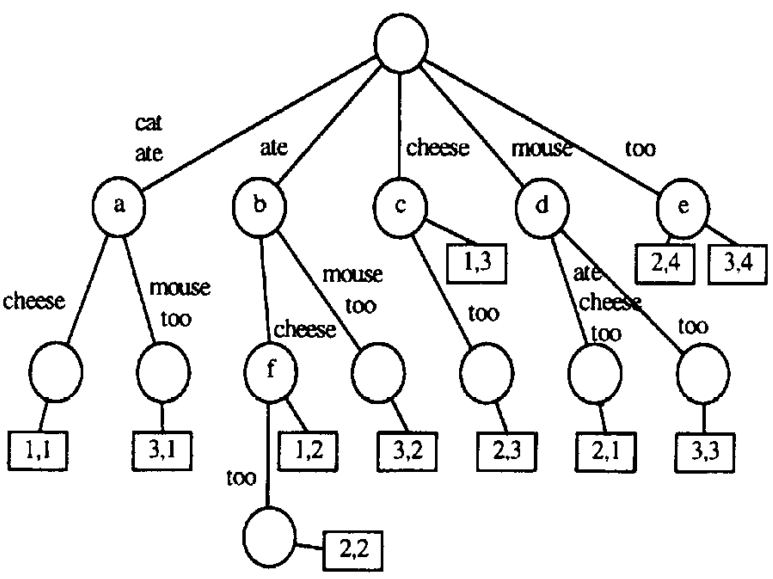
\includegraphics[totalheight=0.3\textheight]{Figures/suffixtree}
  \end{center}
  \caption{A suffix tree generated from the strings “cat ate cheese”, “mouse ate cheese too” and “cat ate mouse too”. From \citetitle{Oren1998} \protect \parencite[p. 48]{Oren1998}}
\end{figure}


\subsection{Compact Trie Clustering}
What is the compact trie clustering algorithm...

\subsection{Performance measures}
What kind of performance measures are used for clustering...

\subsection{Available corpora}
Which corpora are used in clustering and/or classification research? Which ones are suited to clustering? Which ones are used in this master thesis research? Explain scope...


\section{Genetic Algorithms}
\label{GeneticAlgorithm}
General overview of a genetic algorithm here.


\section{Related Work}
\label{RelatedWork}
Introduce related research work in this chapter.